\section{Long Term Monitoring}

\begin{frame}{\PS{} at a Glance}
  \begin{figure}
    \centering
    \begin{tikzpicture}
      \node[anchor=south west,inner sep=0] at (0,0)
      {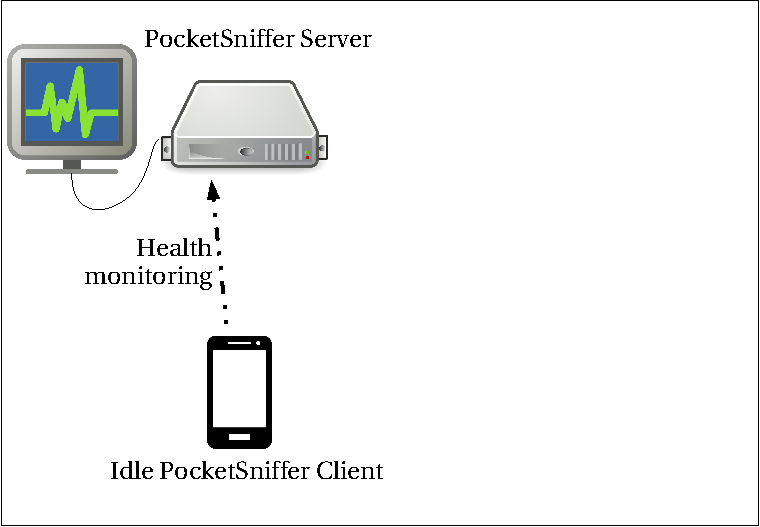
\includegraphics[width=0.6\textwidth]{system-1}};
    \end{tikzpicture}
  \end{figure}
  \textbf{Long-term large scale network monitoring.}
  \begin{itemize}
    \item Network health, performance, etc.
  \end{itemize}
  \color{gray}
  Short-term local spectrum management.
  \begin{itemize}
    \item \color{gray} Sniff the spectrum on behalf of nearby devices.
    \item Help with channel assignment, rate adaption, etc.
  \end{itemize}
\end{frame}


\begin{frame}{\Large Monitoring {\Huge Large} Wireless Network}
  \huge\textbf{\ldots is Hard.}\normalsize
  \begin{block}{If you want to know}
    \begin{itemize}
      \item Whether APs are alive? Easy\textendash SNMP.
      \item How APs are doing? Not so easy.
        \begin{itemize}
          \item \textbf{Client perceived} coverage and performance.
          \item Site surveys? Nay\ldots
        \end{itemize}
    \end{itemize}
  \end{block}
  \huge Smartphones to the rescue!

  \large
  Always on, mostly idle, capture real user experience.
\end{frame}

\begin{frame}{Sounds Good. But\ldots}
  \Large
  \begin{itemize}
    \item \textbf{What} can smartphones measure?
      \begin{itemize}
        \item Monitoring capabilities.
      \end{itemize}
    \item \textbf{How} do we conduct and collect measurements?
      \begin{itemize}
        \item What and When to collect?
      \end{itemize}
    \item \Huge Does this even work?
  \end{itemize}
\end{frame}

\begin{frame}{Smartphone Capabilities}
    What are they already doing?\textendash Network Coverage.
    \begin{itemize}
      \item Wifi scan results (AP visibility and signal quality).
      \item Link quality.
    \end{itemize}
    What can they potentially do?\textendash Network performance.
    \begin{itemize}
      \item Latency.
      \item Bandwidth.
    \end{itemize}
\end{frame}

\begin{frame}{\PS{} Design}
  \begin{block}{Principle}
    \begin{itemize}
      \item Measurements should reflect user's real network experience.
      \item Measurements should not compromise:
      \begin{itemize}
        \item User's interactive usage.
        \item Device's battery life.
      \end{itemize}
  \end{itemize}
  \end{block}
  Smartphones already perform aggressive network exploration.
  \begin{itemize}
    \item Harvesting existing data\textendash take free ride!
  \end{itemize}
  Pay attention to user's \textit{network} activity.
  \begin{itemize}
    \item Trigger performance measurements near them.
  \end{itemize}
  Asynchronous energy-neutral data collection.
  \begin{itemize}
    \item Defer uploads to next charge.
  \end{itemize}
\end{frame}


\begin{frame}{Does it work?\textendash Case Studies}
  Leverage PhoneLab, large scale smartphone testbed at UB.
  \begin{columns}
    \begin{column}{0.7\textwidth}
      \vspace{-3mm}
      \begin{table}
        \centering
        \small
        \begin{tabular}{ccc}
          \toprule
          \textbf{Year} & \textbf{Device} & \textbf{Participant \#} \\\hline
          2012\textendash2013 & Nexus S & 191 \\
          2013\textendash2014 & Galaxy Nexus & 288 \\
          2014\textendash2015 & Nexus 5 & 225\\
          \bottomrule
        \end{tabular}
      \end{table}
    \end{column}
    \begin{column}{0.3\textwidth}
      \vspace{-5mm}
      \begin{figure}
        \centering
        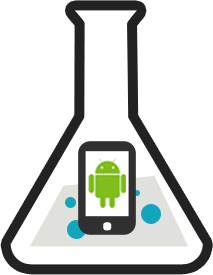
\includegraphics[width=0.4\textwidth]{phonelab_logo_black}
        \caption{\small\url{www.phone-lab.org}}
      \end{figure}
    \end{column}
  \end{columns}
  \begin{block}{PhoneLab Wifi Dataset }
    \begin{itemize}
      \item 139 Android devices over 5 months (11/2013\textendash 3/2014).
      \item 88~M Wifi scan results, 300~K Wifi sessions.
    \end{itemize}
  \end{block}
  \begin{itemize}
    \item Only passive data collection.
    \item This is a \textbf{subset} of what \PS{} would provide (No performance
      measurements).
  \end{itemize}
\end{frame}

\begin{frame}{Android Natural Scan Interval}
  \begin{figure}
    \centering
    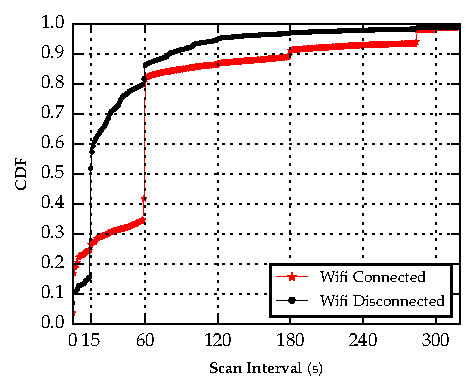
\includegraphics[width=0.6\textwidth]{scan_interval}
  \end{figure}
  \begin{itemize}
    \item 80\% of scan intervals $<$ 1~min.
    \item Justify our free-ride approach.
  \end{itemize}
\end{frame}

\begin{frame}{AP Dominance}
  \begin{figure}
    \centering
    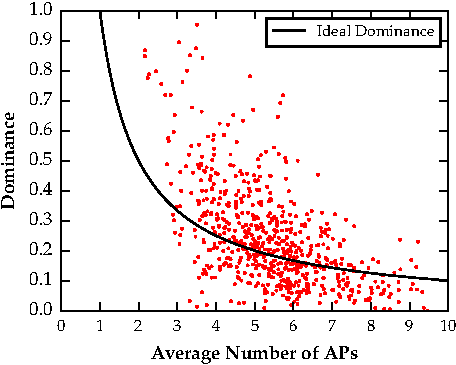
\includegraphics[width=0.6\textwidth]{ap_dominance}
  \end{figure}
  \begin{itemize}
    \item Load balancing is a long way to go.
  \end{itemize}
\end{frame}

\begin{frame}{Signal Coverage}
  \begin{figure}
    \centering
    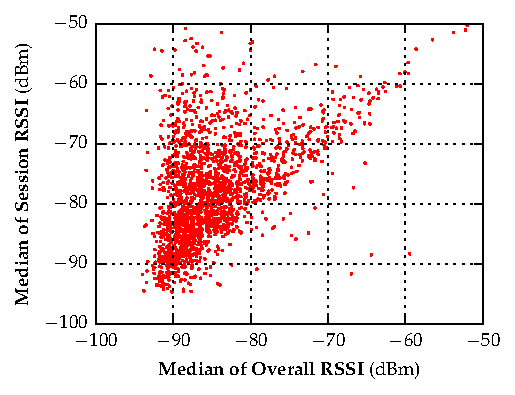
\includegraphics[width=0.6\textwidth]{session_rssi}
  \end{figure}
  \begin{itemize}
    \item User perceived signal coverage may differ from network administrators.
    \item Users tend to adapt their behavior for better signal?
  \end{itemize}
\end{frame}

\begin{frame}{Rogue Access Point}
  \begin{figure}
    \centering
    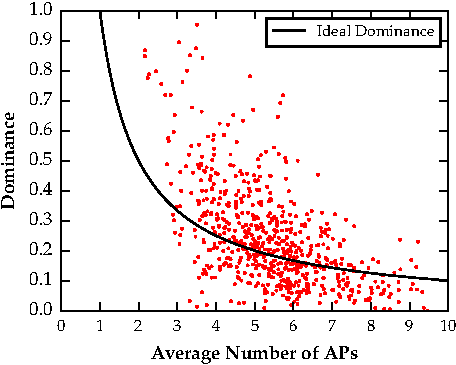
\includegraphics[width=0.6\textwidth]{ap_dominance}
  \end{figure}
  \begin{itemize}
    \item Identify "coverage holes" in campus network.
    \item Rouge AP is not necessarily a bad thing.
  \end{itemize}
\end{frame}
